% !TEX root = labb.tex
\documentclass[conference, onecolumn]{IEEEtran}
\IEEEoverridecommandlockouts%
% The preceding line only needs to identify funding in the first footnote. If that is unnecessary, please comment on it.
\usepackage{cite}
\usepackage{amsmath,amssymb,amsfonts}
\usepackage{algorithmic}
\usepackage{graphicx}
\usepackage{textcomp}
\usepackage{xcolor}
\usepackage{hyperref}
\usepackage{caption}
\usepackage{comment}
\usepackage{colortbl}
\usepackage{booktabs}
\usepackage{tabularx}
\usepackage[most]{tcolorbox}
\usepackage{pdfpages}

\newenvironment{bgquote} {\begin{tcolorbox}[ enhanced, breakable=true, colback=blue!5, colframe=white, boxrule=0pt, left=1em, right=1em, top=0.5em, bottom=0.5em, boxsep=0pt, width=\linewidth, before skip=0.5em, after skip=0.5em ]} {\end{tcolorbox}}

\def\BibTeX{{\rm B\kern-.05em{\sc i\kern-.025em b}\kern-.08em
    T\kern-.1667em\lower.7ex\hbox{E}\kern-.125emX}}

\usepackage{float}

\graphicspath{{../Lab images/}}
\begin{document}

\title{Deep Learning Lab 3 \\
%{\footnotesize \textsuperscript{*}Note: Subtitles should not be used}
}

\author{\IEEEauthorblockN{Suraj Karki}
\IEEEauthorblockA{\textit{Department of Engineering Science }\\
\textit{University West}\\
Trollhättan, Sweden \\
suraj.karki@student.hv.se}
\and
\IEEEauthorblockN{Nils Karlsson}
\IEEEauthorblockA{\textit{Department of Engineering Science }\\
\textit{University West}\\
Trollhättan, Sweden \\
nils.Karlsson@student.hv.se}
\and
\IEEEauthorblockN{Nils Wikström}
\IEEEauthorblockA{\textit{Department of Engineering Science} \\
\textit{University West}\\
Trollhättan, Sweden \\
nils.wikstrom@student.hv.se}
}

\maketitle

\thispagestyle{plain}
\pagestyle{plain}


\begin{IEEEkeywords}
Deep Learning, Laboration 3,
\end{IEEEkeywords}
\begin{abstract} Playing around with learning rate and seeing how it effects performance of NN
\end{abstract}


\section{Task 1}
igure X shows the training and validation accuracy and loss of the CNN over 10 epochs. Both training and validation accuracy increase steadily, reaching 98.4\% and 99.0\%. The training and validation loss decreases without divergence. The validation accuracy remains higher than the training accuracy indicating effective regularization through data augmentation and early stopping, preventing overfitting. The model demonstrates strong generalization performance on the MNIST dataset.
\begin{figure}[htbp]
    \centering
    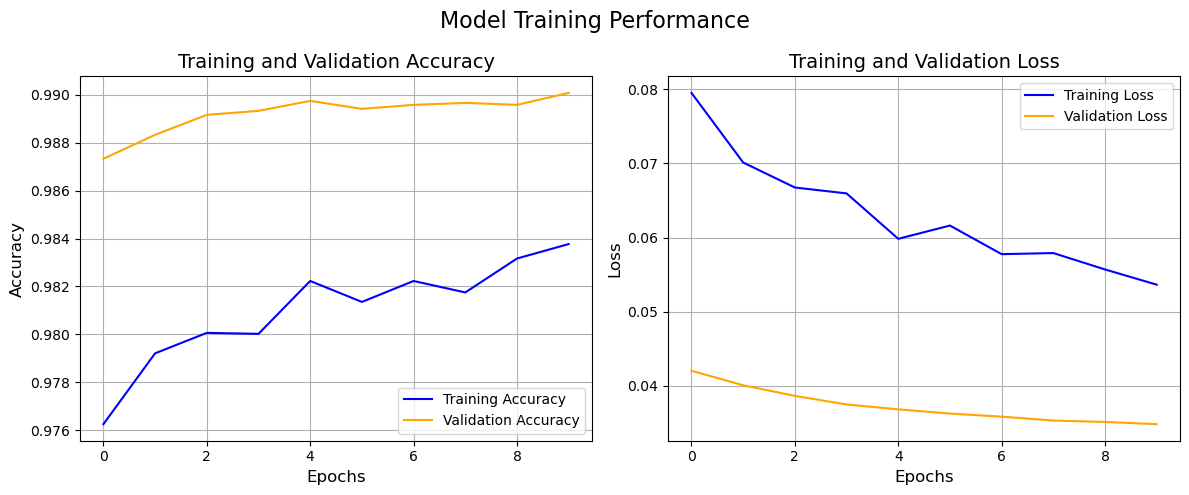
\includegraphics[width=15cm]{model_performance.png}
    \caption{Model Performance on MNIST dataset}
    \label{Model_Performance}
\end{figure}

By usingt Tensorflows Imagegenerator and turning images around or zooming in on them creating more variance of data dropping unnecessary data and implementing eralystops made it so a high precisiong of 98.98\% got achived.
\begin{figure}[htbp]
    \centering
    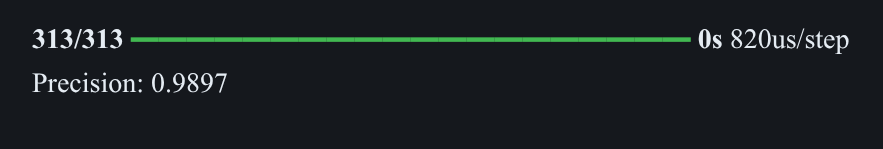
\includegraphics[width=10cm]{precision_Score.png}
    \caption{Precision score}
    \label{Precision output }
\end{figure}
\section{Task 2 }
test 2
\section{Task 3 }
test 3



\bibliographystyle{IEEEtran}
\bibliography{references}

%\textbf{Important for each reference is that it is a clickable doi that makes it easy for a reader to get hold of the reference directly (see examples in bib file).}

\end{document}


